\documentclass[12pt,a4paper]{report}
\usepackage{graphicx}
\usepackage{hyperref}
\usepackage[all]{hypcap}
\usepackage{times}
\usepackage{xcolor}
\usepackage{tabulary}
\usepackage[top=3cm, bottom=3cm, left=3cm, right=2cm]{geometry}
\usepackage{amsmath}
\hypersetup{
    pdftoolbar=true,        % show Acrobat’s toolbar?
    pdfmenubar=true,        % show Acrobat’s menu?
    pdffitwindow=false,     % window fit to page when opened
    pdfstartview={FitH},    % fits the width of the page to the window
    pdftitle={Report of building a wireless communication system},    % title
    pdfsubject={Report},   % subject of the document
    colorlinks,
    linkcolor=violet,
    citecolor=blue,
    urlcolor=brown
}

\begin{document}
    \title{Report of building a wireless communication system}

    \author{course code: B30SQ \\ by Yifei Jing, Xunyu Kai, Zhi Chai}
    \date{April, 2020}
    \maketitle
    \setlength\parindent{0pt}

\chapter{Introduction}
The aim of this project is to build a wireless communication system based on what is learn in the course \emph{B30SQ}.
The structure of a communication system is depicted in \hyperref[fig:system_structure]{Figure \ref*{fig:system_structure}}, which composes of a transmitter and a receiver between two computers.
The transmitter composes of a modulator, a frequency converter, an amplifier, and a patch antenna. The receiver includes a patch antenna, an amplifier, a frequency converter, and a demodulator.
In this project, the modulator is implemented using an integrated USB TTL converter, which simply transform the sequence of 0s and 1s from the computer onto electric signal with 0V indicating 0, and 3.3V indicating 1. The frequency converter is achieved using the integrated module.
The amplifiers contain the Low Noise amplifier designed as the first component to the receiver, the op-amps to provide the second level signal amplification at the receiver and the power amplification at the transmitter.
The type of the antenna is the patch antenna, as the principle is easy to be understood. The frequency converter at the receiver end is implemented using a low pass filer.

\begin{figure}[ht]
    \centerline{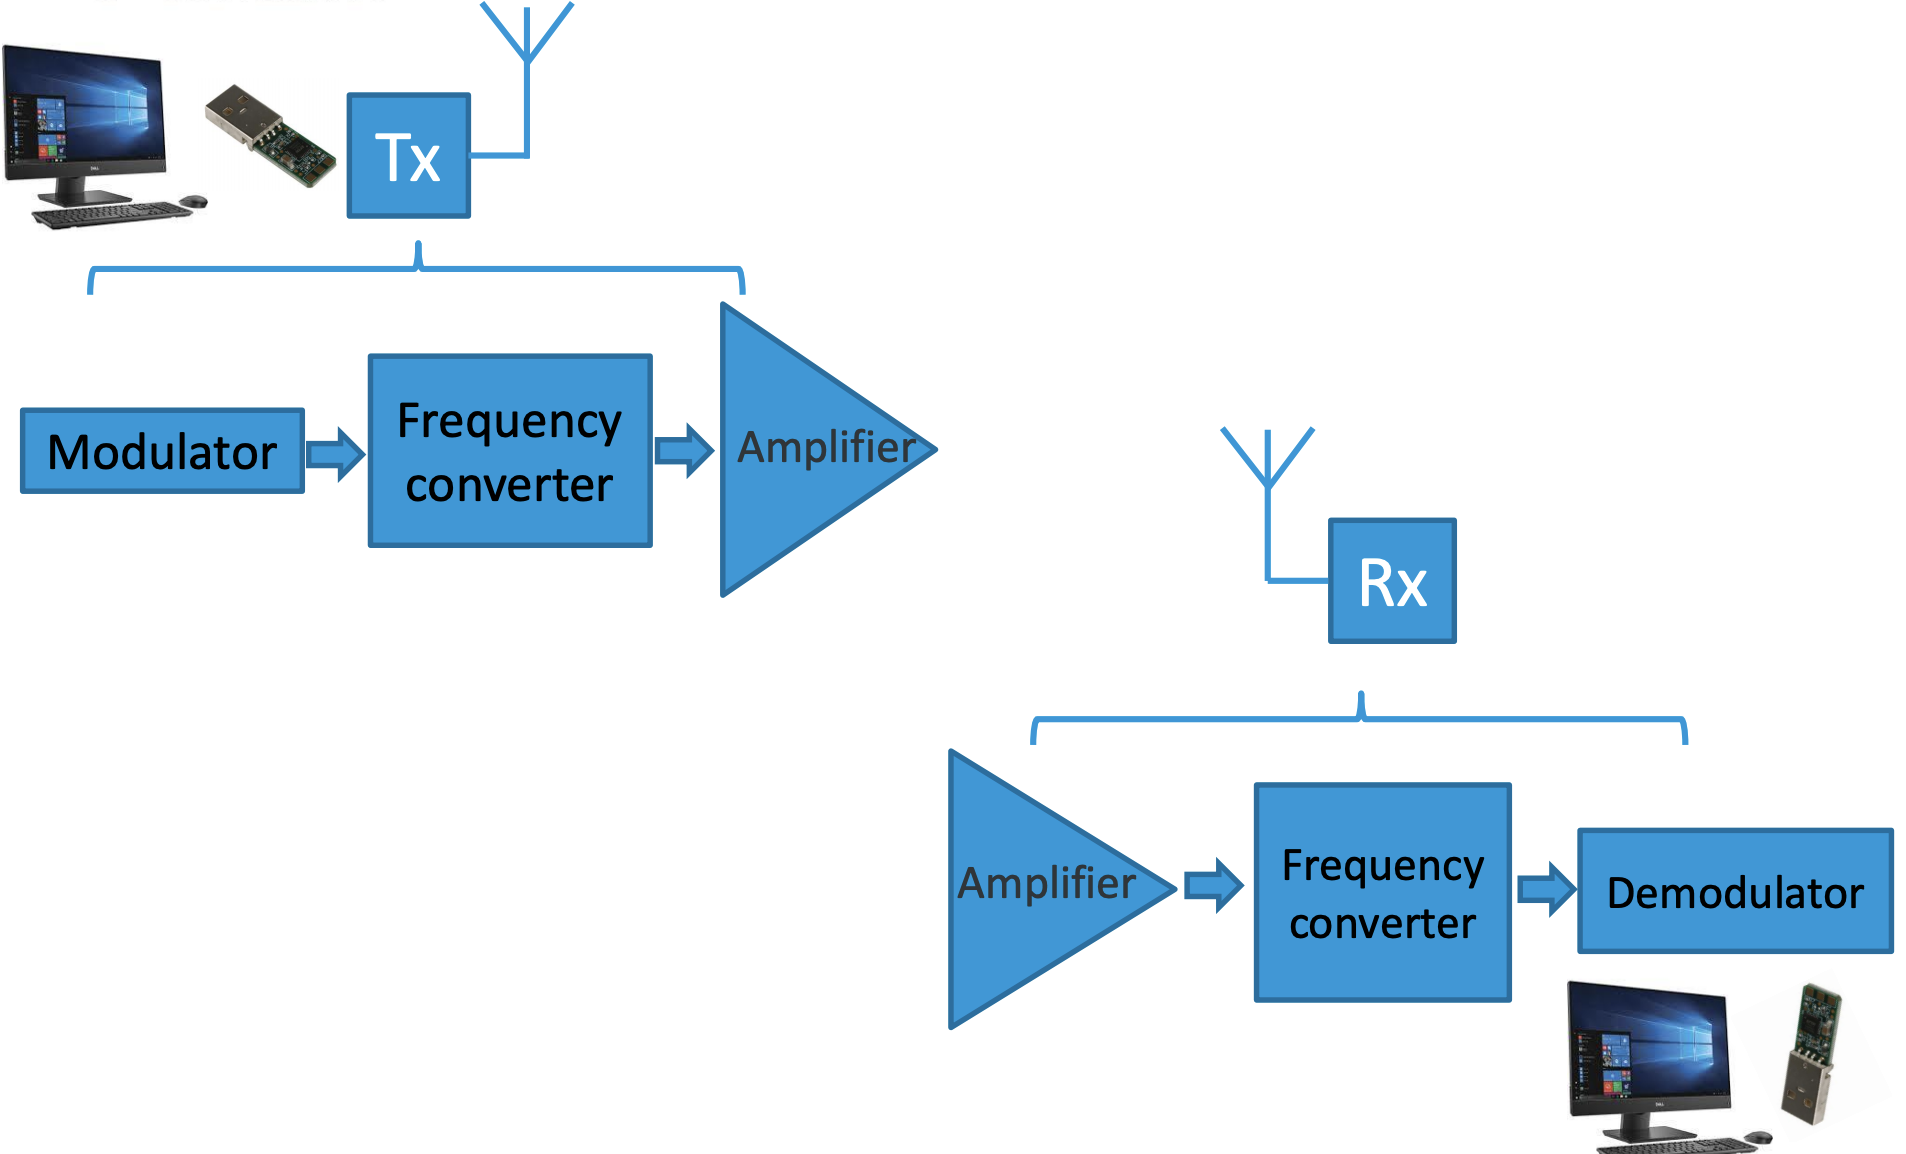
\includegraphics[scale=1]{system_structure}}
    \caption{The structure of a communication system}
    \label{fig:system_structure}
\end{figure}

\section{Operating frequencies}
For the choice of the frequency band, 2400Mhz-2500Mhz is chosen according to ISM: Frequency bands designated for Industrial, Scientific and Medical use.
The reason has been summarized in \hyperref[table:ofea]{Table \ref*{table:ofea}}.

\begin{table}[ht]
    \centering
    \begin{tabulary}{\linewidth}{|L |L| L|}
        \hline
        Frequency band & Standard & Estimation \\ 
        \hline
        433.05 - 434.79 MHz & 5.138 applies. Radiocommunication services must accept harmful interference from ISM. & Antenna size a bit impractical \\
        \hline
        2400 - 2500 MHz & 5.150 applies. Radiocommunication services must accept harmful interference from ISM & Available \\
        \hline
        5725 - 5785 MHz & 5.150 applies. Radiocommunication services must accept harmful interference from ISM. & Elevated cost \\
        \hline
        24.0 - 24.5 GHz & 5.150 applies. Radiocommunication services must accept harmful interference from ISM & Elevated cost and more challenging \\
        \hline
    \end{tabulary}
    \caption{Operating frequencies and estimation of availability}
    \label{table:ofea}
\end{table}

\section{Link budget}
The link budget of a transmitter and a receiver is:
\begin{equation}
    Link \, Budget = L_{FS}(dB) + G_{Tx}(dBi) + G_{Rx}(dBi)
\end{equation}

The term $L_{FS}$ is the free space loss:
\begin{equation}
    L_{FS}(dB) = 32.44 + 20\log{10}{(f(GHz))} + 20\log{10}{(d(meters))}
\end{equation}

Presuming the distance is in the range: $10cm - 2m$, $f = 2.45GHz$, then $L_{FS}$ is in the range $20.2dB - 30.7dB$.
Assuming the gain of the transmitter and the receiver are both $-6dBi$, then the link budget is in the range: $8.2dB - 18.7dB$.
For the requirements that the transmitter and the receiver should be $0dBm$,
\begin{equation}
    P_t(dBm) + G_t(dB) - Link \, Budget + G_r(dB) = P_r(dBm)
\end{equation}
is now re-arranged to: $G_t(dB) + G_r(dB) = Link \, Budget$. Assuming each gain stage is $20dB$, then one stage of amplifier at either transmitter or receiver should be enough.

\chapter{Patch antenna design}
The goal of this section is to design and optimize a quarter-wave matched micro-strip patch antenna fabricated on a FR4 substrate (ER = 4.3, tan(d) = 0.019, thickness = 1.6mm) at about 2.45 GHz.

\section{Concepts}
The principle of design a patched antenna is to achieve a $\lambda / 2$ resonator, as it is illustrated in \hyperref[fig:patch_principle]{Figure \ref*{fig:patch_principle}} that the reflection coefficient is 1 at the open circuit side, and it is approximately 1 on the other side with a thin linked signal feeder.

\begin{figure}[ht]
    \centerline{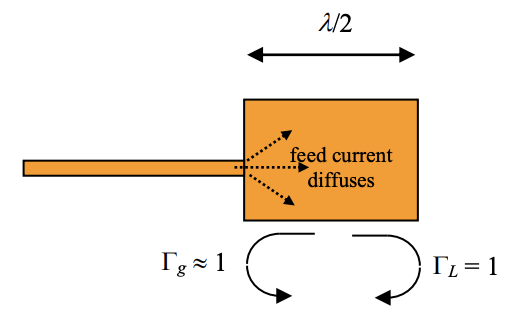
\includegraphics[scale=1.3]{patch_principle}}
    \caption{half-wavelength patch antenna}
    \label{fig:patch_principle}
\end{figure}

Therefore, it is necessary to have the length of the patch equal to $\lambda / 2$. However,  the electric fields are able to extend beyond
the physical edges of the patch as they curl downwards toward the ground plane. This effect called \emph{fringing}, and the result is that the patch appears to be electrically longer than its actual
physical length. Because of this, the required length of the patch, L, is given approximately by
the following equation:
\begin{equation}
    L = \frac{0.49 \lambda_0}{\sqrt{\epsilon_r}}
\end{equation}
where $\epsilon_r$ is the dielectric constant of the substrate, and $\lambda_0$ is the wavelength in free space.

The top view of the patch antenna is shown in \hyperref[fig:top_view]{Figure \ref*{fig:top_view}}, which contains a $50 \Omega$ feed line, a quarter wave transformer, and the square patch with pre-calculated size.

\begin{figure}[ht]
    \centerline{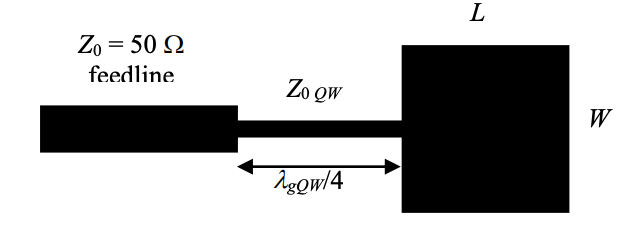
\includegraphics[scale=1.4]{top_view}}
    \caption{The top view of the patch antenna}
    \label{fig:top_view}
\end{figure}

The reason to add the quarter wave transformer is that the input impedance of the patch is very high. The impedance can be represented as \cite{input_impedance}:
\begin{equation}
    R_{IN} \approx 90 (\frac{\epsilon_r^2}{\epsilon_r - 1})(\frac{L}{W})^2
\end{equation}

After calculating the value of $R_{IN}$, the impedance of the quarter wave transformer can be calculated from:

\begin{equation}
    Z_{0QW} = \sqrt{50R_{IN}}
\end{equation}

\vspace{0.2cm}

The characteristic impedance of a transmission line obeys a complicated function of the line width $W$, the substrate height $h$, and the effective dielectric constant $\epsilon_{eff}$. For a given characteristic impedance $Z_0$, the required width of the transmission line is given by:

\begin{equation}
    W = \begin{cases}
        \frac{8h e^A}{e^{2A} - 2} &\text{valid when } W < 2h \\
        \frac{2h}{\pi}[B - 1 - \ln(2B - 1) + \frac{\epsilon_r - 1}{2 \epsilon_r} \{\ln(B - 1) + 0.39 - \frac{0.61}{\epsilon_r}\}] &\text{valid when } W > 2h
    \end{cases}
\end{equation}

\vspace{0.2cm}

where

\begin{equation}
    A = \frac{Z_0}{60} \sqrt{\frac{\epsilon_r + 1}{2}} + \frac{\epsilon_r - 1}{\epsilon_r + 1}\bigg(0.23 + \frac{0.11}{\epsilon_r}\bigg)
\end{equation}
and

\begin{equation}
    B = \frac{377 \pi}{2 Z_0 \sqrt{\epsilon_r}}
\end{equation}

\section{Pre-lab tasks}


\chapter{Amplifier design}
\chapter{Transmitter's modulator}
\chapter{Entire system testing}

\begin{thebibliography}{99}

    \bibitem{input_impedance}
    J.D. Kraus , R.J. Marhafka.
    \textit{Antennas for All Applications, $3^{rd}$ ed.}
    Boston MA: McGraw Hill, 2002, p. 324.

\end{thebibliography}
    
\end{document}